\begin{center}

  \begin{tabular}{rp{16cm}lp{20cm}}%{rl}

  % after \\: \hline or \cline{col1-col2} \cline{col3-col4} ...

  论文地址:& \href{https://arxiv.org/pdf/2006.10637.pdf}{https://arxiv.org/pdf/2006.10637.pdf} \\
  来源:& ICML 2020 Workshop \\
  作者:& Emanuele Rossi, et al. \\
  源码:& \href{https://github.com/twitter-research/tgn}{tgn} \\
  slides:& \href{https://www.emanuelerossi.co.uk/assets/pdf/tgn_aisc_2020.pdf}{TGN: Temporal Graph Networks for Dynamic Graphs} \\
  关键词:& \textbf{graph representation, temporal graph} \\
  写于:& \date{2021-03-01}

  \end{tabular}

\end{center}

该论文\cite{rossi2020temporal}主要解决的是连续时间下的动态图的表示,论文中将连续时间下的动态图看成流图 --- 由一系列的带时间戳的事件组成。

\paragraph{问题定义}
论文中将动态图建模为带时间戳的事件序列:$\mathcal{G}=\left\{x\left(t_{1}\right), x\left(t_{2}\right), \ldots\right\}$。事件$x(t)$有两种类型:1)结点事件,新增一个结点或者更新一个结点的特征,用$\mathbf{v}_i(t)$表示;2)交互事件:表示结点之间的交互,由$\mathbf{e}_{i j}(t)$表示。该论文的主要贡献就是建立了一个通用的框架来对动态图进行建模,并且将一系列的模块组合起来对动态图进行学习,得到结点在某个时间点上的表征。\textbf{将TGN作用在一个连续时间的动态图上,将为每个结点在每个时间点上产生一个表征}。

\paragraph{TGN思路}
简言之,TGN可以看作一个编码器,共由5个子模块组成。

\subparagraph{Memory}
$t$时的模型的Memory由模型到$t$时为止所见到的结点$i$的状态$\mathbf{s}_i(t)$组成。结点的状态相当于对结点的历史信息的一个压缩形式的表示。

\subparagraph{Message Function}
$t$时,当有涉及$i$结点的事件时,一条message会被计算用于更新$i$的状态。论文中对两种事件的消息计算公式如下:
$$
\mathbf{m}_i(t) = msg_s(\mathbf{s}_i(t^{-}), \mathbf{s}_j(t^{-}), \triangle t, \mathbf{e}_{ij}(t))
$$
$$
\mathbf{m}_j(t) = msg_d(\mathbf{s}_j(t^{-}), \mathbf{s}_i(t^{-}), \triangle t, \mathbf{e}_{ij}(t))
$$
$$
\mathbf{m}_i(t) = msg_n(\mathbf{s}_i(t^{-}), t, \mathbf{v}_{i}(t))
$$

$msg_s, msg_t, msg_n$分别表示交互事件中源节点和目标节点、结点事件中所涉及的结点的消息的计算公式。具体实现时可以有多种形式,如MLP,在论文中采用的是拼接的形式。

\subparagraph{Message Aggregator}
由于在实际中通常会采用一次性处理多个事件(可能是多个时间的多个事件),需要将多个事件对应的message汇聚,形式如下:
$$
\bar{\mathbf{m}}_i(t) = agg(\mathbf{m}_i(t_1), ..., \mathbf{m}_i(t_b))
$$
$agg$的具体实现形式也可以是多样的,如RNN、mean等,论文中采用的是只选择最近的message。

\subparagraph{Memory Updater}
得到了$t$时设计到$i$的message后就可以更新状态了。
$$
\mathbf{s}_i(t) = mem(\bar{m}_i(t), \mathbf{s}_i(t^-))
$$
同样,$mem$的形式也可以是多样的,如LSTM、GRU等。

\subparagraph{Embeddings}
这个模块是用于为$i$生成在$t$时的表征的:
$$
\mathbf{z}_i(t) = emb(i, t) = \sum_{j \in N_i^k([0, t])} h(\mathbf{s}_i(t), \mathbf{s}_j(t), \mathbf{e}_{ij}, \mathbf{v}_i(t), \mathbf_{v}_j(t))
$$
$h$的具体形式也是多样的。

最终TGN的整体如Fig.\ref{fig:tgn}所示。
\begin{figure}[h]
	\centering
	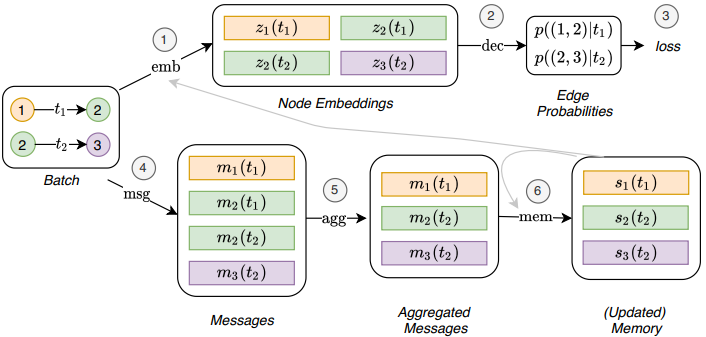
\includegraphics[width=.8\textwidth]{pics/TGN.png}
	\caption{TGN}
	\label{fig:tgn}
\end{figure}



\paragraph{方法解决的问题/优势}

\begin{itemize}

	\item 对连续时间下的动态图进行了建模,以事件序列表示一个动态图
	\item 对动态图的表征学习提出了一个统一的框架
	\item 可应用于异常检测、金融交易等场景中
	
\end{itemize}

